\section{The Dirac equation and anti-particles}
Last year you saw processes of the form:
$e^+e^-\to \mu^+\mu^-$ or $e^+e^-\to q\bar{q}$ where $e^+$ is the anti-particle
of the $e^-$, $\mu^+$ the anti-particle of the $\mu^-$ and $\bar{q}$ the anti-particle of $q$. However, so far the Schr\"odinger equation says nothing about anti-particle states. 

\begin{figure}
\caption{Paul A.M.~Dirac}
\begin{tabular}{cc}
\parbox{0.32\textwidth}{
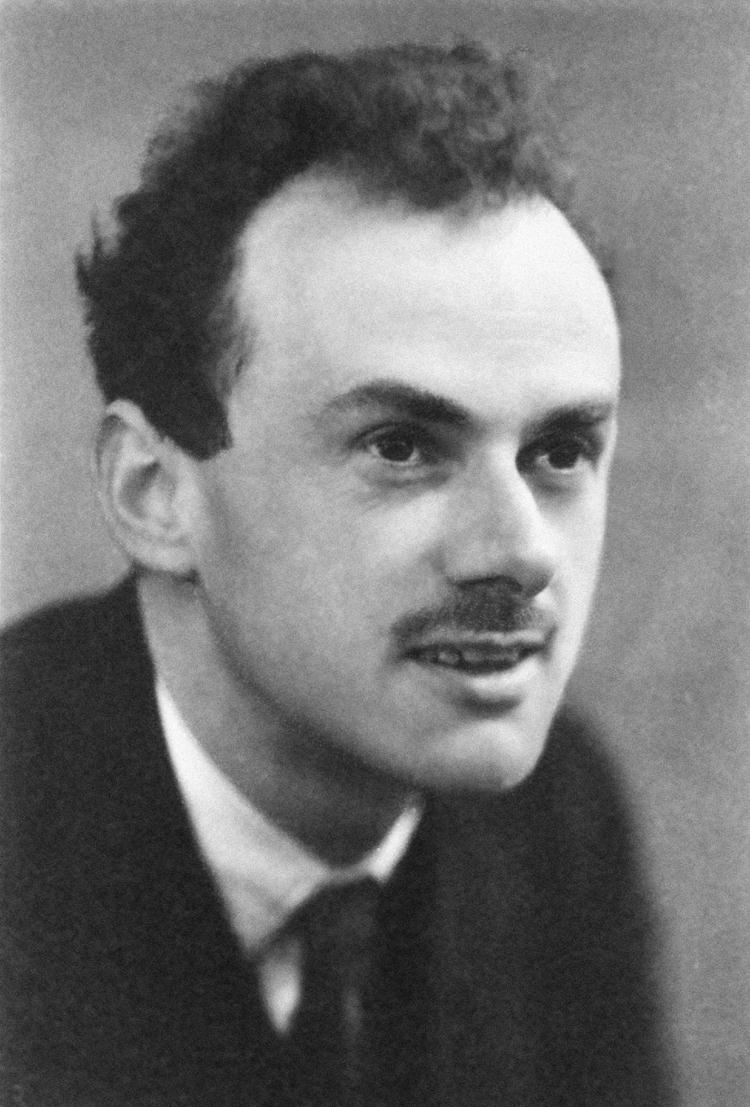
\includegraphics[width=0.3\textwidth]{fig/dirac/Dirac_4.jpg}
}&
\parbox{0.66\textwidth}{\textsf{\small
    ``Paul A.M.~Dirac studied Electrical engineering and Mathematics at the {\bf University of Bristol} before going to Cambridge for his PhD. In 1928 he developed a relativistic form of the wave equation which implied the existence of anti-matter and also provided theoretical justification for intrinsic angular momentum (spin). He was awarded the Nobel Prize in 1933 together with Schr\"odinger.'' 
}}
\end{tabular}
\\  \textsf{Source: \httplink{https://en.wikipedia.org/wiki/Paul\_Dirac}}
\end{figure}

In fact the main problem with the Schr\"odinger is that in its current form it does not account for relativistic effects. Dirac tried to address this issue in order to understand relativistic effects in the hydrogen atom. 

\paragraph{The Hydrogen atom}
Consider the hydrogen atom whose energy levels are given by
\[
|E_n|=\left(\frac{e^2}{4\pi\epsilon_0}\right)^2\frac{m_{e}}{2\hbar^2}\frac{1}{n^2}.
\]
Equating this energy to the kinetic energy of the electron (Virial theorem) we arrive at the expression:
\[
v_{e}\sim \frac{e^2}{4\pi\epsilon_0\hbar}=\frac{c\alpha}{n^2},
\]
\noindent where $\alpha=\frac{1}{137}$ is the fine-structure constant.
Therefore at the ground state ($n=1$), the electron speed is $\sim 1\%$ of the speed of light so relativistic effects start to have a small but measurable effect.

\subsection{Towards a relativistic form of Schr\"odinger's equation}

Schr\"odinger's equation in 3 dimensions for a free massive particle is given by:
\begin{equation}
\label{eq:schrodinger_free_massive}
-\frac{\hbar^2}{2m}\vec{\nabla}^2\psi=i\hbar\frac{\partial\psi}{\partial t}
\end{equation}
It can be shown that this equation is not Lorentz-covariant ie under a Lorentz transformation, Eq.~\ref{eq:schrodinger_free_massive} does not hold in all inertial frames. In other words, it cannot be written in terms of 4-vector or scalar quantities.

An easy way of seing this, is that the left-hand-side of Eq.~\ref{eq:schrodinger_free_massive} has a $2^{\rm nd}$ order space derivative but the right-hand-side has a $1^{\rm st}$ order time derivative.

\paragraph{Momentum and Energy operators}
The solution to Eq.~\ref{eq:schrodinger_free_massive} can be written as
\[
\psi(\vec{x},t)\propto e^{i(\vec{k}\cdot\vec{x}-\omega t)}.
\]
By inserting into Eq.~\ref{eq:schrodinger_free_massive} one ends up with the relation:
\[
\frac{p^2}{2m}\psi=E\psi.
\]
By inspection therefore we can write\footnote{Note that a more formal derivation of these operators exists by considering the effect of infinitesimal translations of space and time.}:
\begin{eqnarray}
\label{eq:mom_operator}
\hat{p}=-i\hbar\vec{\nabla}\\
\hat{E}=i\hbar\frac{\partial}{\partial t}.
\end{eqnarray}

\subsection{The Klein-Gordon equation}
We also know from relativity that $E^2=m^2c^4+p^2c^2$. Therefore using our momentum and energy operators above, we can write an alternative to Schr\"odingers equation that is inherently relativistic, as we have started from the relativistic relation between energy and momentum ie
\begin{equation}
\label{eq:klein_gordon}
(\frac{1}{c^2}\frac{\partial^{2}}{\partial t^2}-\vec{\nabla}^2)\psi+\frac{m^2c^2}{\hbar^2}\psi=0
\end{equation}
This is known as the Klein-Gordon equation. As you can now see the spatial derivatives and time derivatives are of the same order. Actually if you look close enough you will notice that what we have written, CAN be arranged in terms of 4-vectors and scalars. Consider the 4-vector: $\nabla=(\frac{1}{c}\frac{\partial}{\partial t},\frac{\partial}{\partial \vec{x}})$. We can therefore write Eq.~\ref{eq:klein_gordon} as
\begin{equation}
\label{eq:klein_gordon_2}
(\nabla\cdot\nabla)\psi+\frac{m^2c^2}{\hbar^2}\psi=0
\end{equation}
Therefore Eq.~\ref{eq:klein_gordon_2} is Lorentz covariant.

Great, so we have arrived at a relativist form of Eq.~\ref{eq:schrodinger_free_massive}. However, we have one major problem. It turns out that the solutions of the Klein-Gordon equation give a probability density that is negative. The probability density of the Schr\"odinger equation is given by
\[\rho=|\psi|^2=\psi^\dagger\psi\]. 
The equivalent expression for the Klein-Gordon equation is 
\[\rho=\pm 2\sqrt{p^2c^2+m^2c^4}|\psi|^2.\]
The fact that the Klein-Gordon equation can return negative probability density solutions was originally a true killer of this approach. The Klein-Gordon equation also returns negative energy solutions which means that an interacting particle could radiate away an infinite amount of energy while cascading to an infinitely low energy state. However with the advent of Quantum Field Theory, the negative probability solutions could be understood and therefore the Klein-Gordon equation was restored as a genuine description of relativistic massive particles with no spin. 

\exercise{ (beyond scope) The continuity equation is given by:
\begin{equation}
\label{eq:continuity_equation}
\frac{\partial\rho}{\partial t}+\vec{\nabla}\vec{j}=0,
\end{equation}
where $\rho$ represents a quantity per unit volume  (e.q charge density) and $j$ is the flux of that quantity (e.g current per unit area flowing through a surface).
In quantum mechanics the continuity equation expresses the flow of probability in complete analogy to electromagnetism or fluid mechanics. The flux in this case is the probability per unit time per unit area that the particle will pass through a surface. The continuity equation in quantum mechanics reflects the fact that a particle moves through space in a continuous manner and that the integral of  the probability distribution of its position over all space is always 1.

By rewriting the Klein-Gordon equation to look like the continuity equation  show that the probability density $\rho$ is given by 
\[
\rho=\pm 2\sqrt{p^2c^2+m^2c^4}|\psi|^2.
\]
Hint: take complex conjugate of Eq.~\ref{eq:klein_gordon} and  multiply both left and right-hand side by $\psi$). Also multiply both left and right-hand side of Eq.~\ref{eq:klein_gordon} by $\psi^*$.
}

In any case, for what concerns us and also Dirac, the Klein-Gordon equation has this unwanted feature of negative probability density solutions.

\subsection{The Dirac equation}
In order to avoid the negative probability solution, Dirac wanted the relativistic form of Schr\"odinger's equation to be $1^{\rm st}$ order in the time derivative and maintain its Lorentz-covariance. These requirements meant that the equation should look something like (using natural units for simplicity):
\begin{equation}
\label{eq:dirac_template}
i\alpha^0\frac{\partial\psi}{\partial t}=m\psi-i\vec{\alpha} \vec{\nabla}\psi,
\end{equation}
where $\alpha^0$ and $\vec{\alpha}$ are a set of constants.
These constants can be determined by requiring that 
\begin{equation}
\label{eq:dirac_constraint}
[\alpha^0\hat{E}-\vec{\alpha}\hat{p}+m][\alpha^0\hat{E}-\vec{\alpha}\hat{p}-m]\psi=[\hat{E}^{2}-\hat{p}^2-m^2]\psi
\end{equation}
ie requiring that Eq.~\ref{eq:dirac_template} is compatible with the Klein-Gordon equation and is therefore relativistic. Note that again for simplicity we have used the energy and momentum operators (see Eq.~\ref{eq:mom_operator}) to represent the time and spatial derivatives respectively.

\exercise{ (beyond scope) Show that:
\begin{equation*}
\alpha^{\mu}\alpha^{\nu}+\alpha^{\nu}\alpha^{\mu}=0
\end{equation*}
for $\mu\neq\nu$, where $\mu,\nu=0,1,2,3$. Hence show that these $\alpha$'s cannot be normal numbers.
Also show that:

\begin{eqnarray*}
(\alpha^{0})^{2}=I\\
(\alpha^{i})^{2}=-I
\end{eqnarray*}
where $I$ is the unit matrix.
}\\\\

It turns out that the only way Eq.~\ref{eq:dirac_constraint} can hold, is if $a^0$ and $\vec{\alpha}$ are matrices. The smallest size matrices that satisfy Eq.~\ref{eq:dirac_constraint} are $4\times4$ and they are generally called the $\gamma=(\gamma^0,\vec{\gamma})$-matrices and are not not to be confused with the boost factor $\gamma$.
The Dirac equation is therefore written as:
\begin{equation}
\label{eq:dirac_equation}
i\gamma^0\frac{\partial\psi}{\partial t}+i\vec{\gamma}\cdot \vec{\nabla}\psi-m\psi=0
\end{equation}
A standard form of the $\gamma$-matrices can be given by:
\begin{equation}
\gamma^0=\mII{I}{0}{0}{-I}, \gamma^1=\mII{0}{\sigma^1}{-\sigma^1}{0},
\gamma^2=\mII{0}{\sigma^2}{-\sigma^2}{0},
\gamma^3=\mII{0}{\sigma^3}{-\sigma^3}{0},
\end{equation}
where $I$ is a $2\times2$ unit-matrix and $\sigma^{1,2,3}$ are the well known Pauli-matrices.
The hermition conjugates of the $\gamma$-matrices follow:
\begin{equation}
\gamma^{0\dagger}=\gamma^0,\gamma^{1\dagger}=-\gamma^1,\gamma^{2\dagger}=-\gamma^2,\gamma^{3\dagger}=-\gamma^3
\end{equation}

The benefit of Dirac's approach is that the probability density is always positive as it is given by:
\[
\rho=\psi^\dagger\psi=|\psi|^2
\]
Note that as we shall see in the next section, $\psi$'s are now column vectors therefore the hermitian conjugate is required rather than just the complex conjugate.

\exercise{ (beyond scope) Just as for the Klein-Gordon equation, rewrite the Dirac equation to look like the continuity equation (Eq.~\ref{eq:continuity_equation}) to show that the probability density $\rho$ is given by 
\[
\rho=\psi^\dagger\psi=|\psi|^2
\]
Hint: take the hermitian conjugate of Eq.~\ref{eq:dirac_equation} and  multiply both left and right-hand side by $\psi$. Also multiply both the left and right hand side of Eq.~\ref{eq:dirac_equation} by $\psi^\dagger\gamma^0$)
}

\subsection{Solutions to the Dirac equation}
For simplicity lets assume $\nabla\psi=0$ (particle at rest). In this case the solutions to Eq.~\ref{eq:dirac_equation} are given by
\begin{eqnarray}
\psi^{(1)}=e^{-i\frac{mc^2}{\hbar}t}\vIV{1}{0}{0}{0},
\psi^{(2)}=e^{-i\frac{mc^2}{\hbar}t}\vIV{0}{1}{0}{0}\\
\psi^{(3)}=e^{+i\frac{mc^2}{\hbar}t}\vIV{0}{0}{1}{0},
\psi^{(4)}=e^{+i\frac{mc^2}{\hbar}t}\vIV{0}{0}{0}{1}.
\end{eqnarray}
Note we have written the solutions down using SI units in order to help us understand what is going on.

There are two important aspects here
\begin{enumerate}
\item We have exponents with two signs $+\frac{mc^2}{\hbar}t$ and $-\frac{mc^2}{\hbar}t$. These correspond to two energy solutions $E=-mc^2$ and $E=+mc^2$ respectively.
\item The solution is in a form of a vector. We can recognise two patterns: $\vII{1}{0}$ and $\vII{0}{1}$. These correspond to spin-up and spin-down respectively.
\end{enumerate}
What does this all mean? Dirac interpreted the negative energy solutions by postulating the existence of a sea of negative energy states. The vacuum, or ground state, has all the negative energy states full. An additional electron must therefore occupy the positive energy state, as Pauli's exclusion principle forbids it from falling into one of the filled negative energy states. On promoting one of the negative energy states to a positive energy state by supplying energy, an electron-hole pair is created, ie a positive energy electron and a negative energy hole (the hole lying in the negative energy sea). The hole is therefore seen as a positron (anti-electron) of positive energy. The major problem with this approach however, is that it only works for fermions and not bosons as the Pauli exclusion principle does not apply. Nevertheless since Dirac's equation describes spin-1/2 objects, his interpretation is not completely incorrect. 

A more modern interpretation by Feynman and Stueckelberg, suggests that negative energy particles are equivalent to positive energy particles travelling backwards in time ie can require that 
\[
e^{-i\frac{-mc^2}{\hbar}t}=e^{-i\frac{mc^2}{\hbar}(-|t|)}
\]
avoiding the argument requiring Pauli's exclusion principle!

We have been banging on about the Dirac equation describing spin-1/2 objects. Well it takes a bit more work to prove this. A full formal proof is beyond the scope of this course however we can try to see how this statement comes about.

\subsection{General solutions to the Dirac equation and spin}

It can be shown (though beyond the scope of this course) that the general solutions of the Dirac equation for a moving particle of mass $m$ with momentum $\vec{p}$ are given: for $E>0$
   
\[\psi^{(1)}(\vec{r},t)=\sqrt{|E|+m}  e^{-i(Et-\vec{p}\cdot\vec{r})}
\vIV{1}{0}{\frac{p_z}{(E+m)}}{\frac{p_x+ip_y}{E+m}},
\psi^{(2)}(\vec{r},t)=\sqrt{|E|+m}
e^{-i(Et-\vec{p}\cdot\vec{r})}\vIV{0}{1}{\frac{p_x-ip_y}{(E+m)}}{\frac{-p_z}{E+m}},
\] 
and for $E<0$
\[
\psi^{(3)}(\vec{r},t)=\sqrt{|E|+m}  e^{-i(Et-\vec{p}\cdot\vec{r})}
\vIV{\frac{p_z}{(E-m)}}{\frac{p_x+ip_y}{(E-m)}}{1}{0},
\psi^{(4)}(\vec{r},t)=\sqrt{|E|+m}  e^{-i(Et-\vec{p}\cdot\vec{r})}
\vIV{\frac{-p_z}{(E-m)}}{\frac{p_x-ip_y}{(E-m)}}{0}{1}.
\] 

These solutions to the Dirac equation are also eigenstates of the Hamiltonian operator given by
\[
 \hat{H} = \gamma^{0}(\gamma^1\hat{p}_x+ \gamma^2\hat{p}_y + \gamma^3\hat{p}_z)+\gamma^{0}m, 
\]
where $\hat{p}_{x,y,z}$ are momentum operators.
By considering the orbital angular momentum operator 
\[\hat{\vec{L}} =
\vIII{y\hat{p}_z-z\hat{p}_y}{z\hat{p}_x-x\hat{p}_z}{x\hat{p}_y-y\hat{p}_x},\]
and remembering that the only non zero commutators of position and momentum are 
\[ [x,\hat{p}_x] = [y,\hat{p}_y] =  [z,\hat{p}_z] =
  i, 
\]
we can show that ({\bf see problem sheet 2})\[
[\hat{H},\hat{\vec{L}}] =
-i\gamma^{0}\vIII{\gamma^2\hat{p}_z-\gamma^3\hat{p}_y}{\gamma^3\hat{p}_x-\gamma^1\hat{p}_z}{\gamma^1\hat{p}_y-\gamma^2\hat{p}_x}\neq\vec{0}
\]

This is quite an interesting result as it implies that orbital angular momentum is not conserved. We can explain this by requiring that the orbital angular momentum is not the complete picture. There should be another component of angular momentum intrinsic to the state itself, which when added to the orbital angular momentum, the total sum is conserved. That is the sum

\[\hat{\vec{J}}=\hat{\vec{L}}+\hat{\vec{\Sigma}},\]

where $\hat{\vec{\Sigma}}$ is the spin operator of our states $\psi^{(1-4)}$, does commute with the Hamiltonian. 

Furthermore, we can extend the concept of the spin operator you learned about in your 3rd year Quantum Mechanics course to be applicable to these 4-component $\psi$ states:

In your QM course you demonstrated that the spin operators can be written in terms of the Pauli matrices (in natural units) as 
\[
\hat{S}_x=\frac{1}{2}\sigma_1,\hat{S}_y=\frac{1}{2}\sigma_2,\hat{S}_z=\frac{1}{2}\sigma_3
\]

However as the solutions to the Dirac equation have four components representing particle/anti-particle states of spin-up and spin-down we extend the Spin operators from 2D matrices to 4D as


\[ \hat{\Sigma}_{x} =1/2
\mII {\sigma_{1}}{\underline{0}}{\underline{0}}{\sigma_{1}} ,
\hat{\Sigma}_{y} =1/2
\mII {\sigma_{2}}{\underline{0}}{\underline{0}}{\sigma_{2}} ,
\hat{\Sigma}_{z} =1/2
\mII {\sigma_{3}}{\underline{0}}{\underline{0}}{\sigma_{3}}.
\]

where $\underline{0}$ is the $2\times2$ null-matrix 
$\mII{0}{0}{0}{0}$.

Now we can easily show ({\bf see problem sheet 2}) that the states $\psi^{(1-4)}$ are not eigenstates of the spin operator $\hat{\Sigma}_{z}$. This should be easily understood as the solutions to the Dirac equation are also eigenstates of the Hamiltonian. Therefore it is the total angular momentum $J_z$ that is conserved and not the individual $L_z$ or $S_z$ values.

However, in the case that the momentum of the particle is pointing only in the $z$-direction, then 
it can be easily shown that ({\bf see problem sheet 2})
\[
\hat{\Sigma}_{z}\psi^{(1,3)}=\frac{1}{2}\psi^{(1,3)},\\
\hat{\Sigma}_{z}\psi^{(2,4)}=-\frac{1}{2}\psi^{(2,4)},
\]
for the case that $p_x=p_y=0$. This result therefore suggests that the Dirac equation describes particles with $\Sigma_{z}=\pm\frac{1}{2}$

Also note that the states  $\psi^{(1-4)}$ are eigenstates of the total spin operator
\[
\hat{\vec{\Sigma}}^2=\hat{\vec{\Sigma}}^{\dagger}\hat{\vec{\Sigma}}
\]
with eigenvalue $\Sigma^2=\frac{3}{4}$

\exercise{Show that $\hat{\vec{\Sigma}}^{2}=3/4$ where $I$ is a $2\times2$ unit matrix. Hint: use the property of the Pauli matrices that $\sigma_{i}^{\dagger}\sigma_{i}=I$}

To summarise, Dirac's equation describes spin-1/2 particles and their anti-particle partner. For example for electrons and positrons we have:

\begin{eqnarray*}
\psi^{(1)}\equiv e^- {\rm spin}-1/2 \uparrow,
\psi^{(2)}\equiv e^- {\rm spin}-1/2 \downarrow\\
\psi^{(3)}\equiv e^+ {\rm spin}-1/2 \uparrow, \psi^{(4)}\equiv e^+ {\rm spin}-1/2 \downarrow.
\end{eqnarray*}
